\documentclass[12pt,letterpaper]{article}
\usepackage{graphicx,textcomp}
\usepackage{natbib}
\usepackage{setspace}
\usepackage{fullpage}
\usepackage{color}
\usepackage[reqno]{amsmath}
\usepackage{amsthm}
\usepackage{fancyvrb}
\usepackage{amssymb,enumerate}
\usepackage[all]{xy}
\usepackage{endnotes}
\usepackage{lscape}
\newtheorem{com}{Comment}
\usepackage{float}
\usepackage{hyperref}
\newtheorem{lem} {Lemma}
\newtheorem{prop}{Proposition}
\newtheorem{thm}{Theorem}
\newtheorem{defn}{Definition}
\newtheorem{cor}{Corollary}
\newtheorem{obs}{Observation}
\usepackage[compact]{titlesec}
\usepackage{dcolumn}
\usepackage{tikz}
\usetikzlibrary{arrows}
\usepackage{multirow}
\usepackage{xcolor}
\newcolumntype{.}{D{.}{.}{-1}}
\newcolumntype{d}[1]{D{.}{.}{#1}}
\definecolor{light-gray}{gray}{0.65}
\usepackage{url}
\usepackage{listings}
\usepackage{color}

\definecolor{codegreen}{rgb}{0,0.6,0}
\definecolor{codegray}{rgb}{0.5,0.5,0.5}
\definecolor{codepurple}{rgb}{0.58,0,0.82}
\definecolor{backcolour}{rgb}{0.95,0.95,0.92}

\lstdefinestyle{mystyle}{
	backgroundcolor=\color{backcolour},   
	commentstyle=\color{codegreen},
	keywordstyle=\color{magenta},
	numberstyle=\tiny\color{codegray},
	stringstyle=\color{codepurple},
	basicstyle=\footnotesize,
	breakatwhitespace=false,         
	breaklines=true,                 
	captionpos=b,                    
	keepspaces=true,                 
	numbers=left,                    
	numbersep=5pt,                  
	showspaces=false,                
	showstringspaces=false,
	showtabs=false,                  
	tabsize=2
}
\lstset{style=mystyle}
\newcommand{\Sref}[1]{Section~\ref{#1}}
\newtheorem{hyp}{Hypothesis}

\title{Final Project}
\author{Caroline Kajkowski}

\begin{document}
	\maketitle
	
\subsection*{Data Story and Manipulation}
\begin{description}
	\item[The Data] description
\end{description}
	\lstinputlisting[language=R, firstline=24, lastline=51]{final_project.R}  

\subsection*{Data Visualization}
\title{Visualization 1}
	\lstinputlisting[language=R, firstline=55, lastline=85]{final_project.R}  
		\begin{figure}[H]
		\centering
		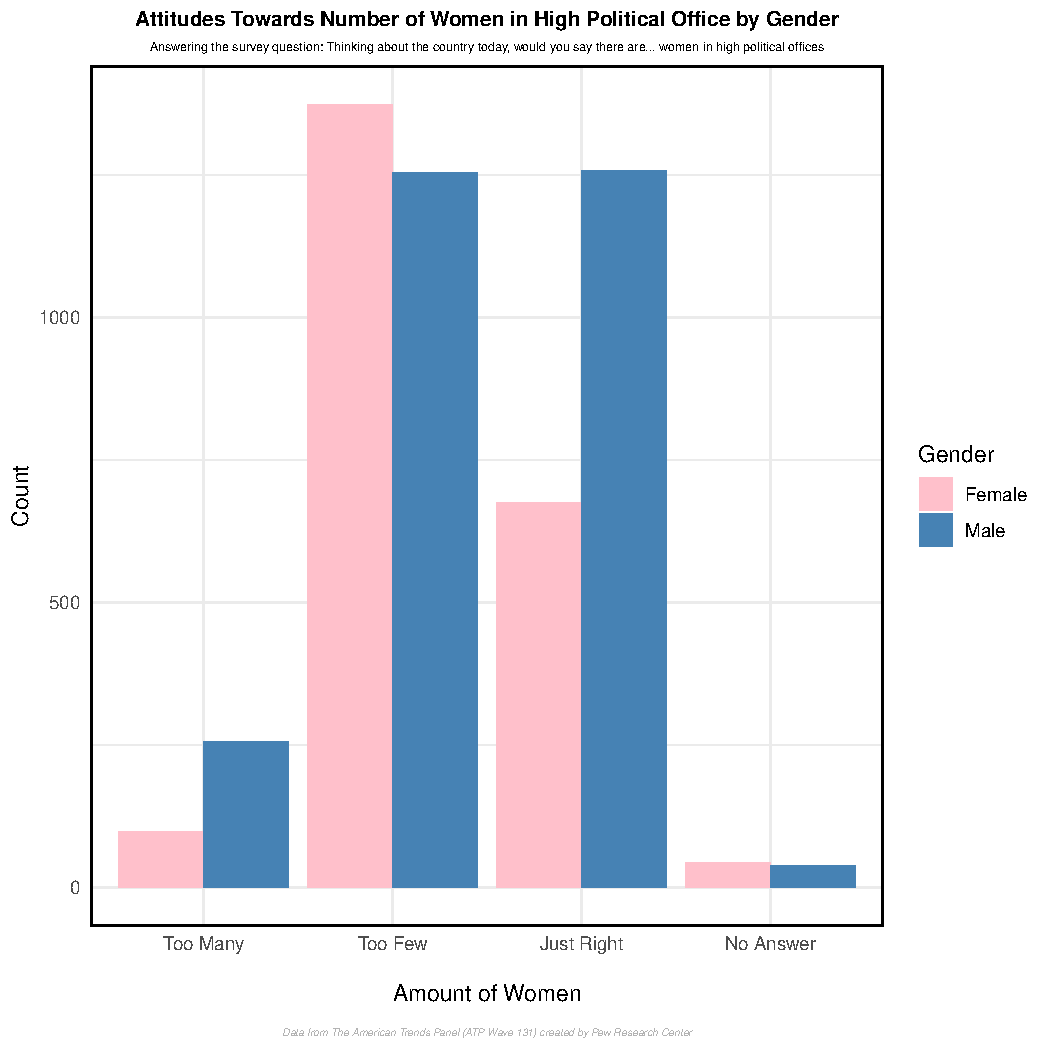
\includegraphics[width=0.9\textwidth]{bar.pdf}
	\end{figure}


\title{Visualization 2}
\lstinputlisting[language=R, firstline=87, lastline=133]{final_project.R}  
\begin{figure}[H]
	\centering
	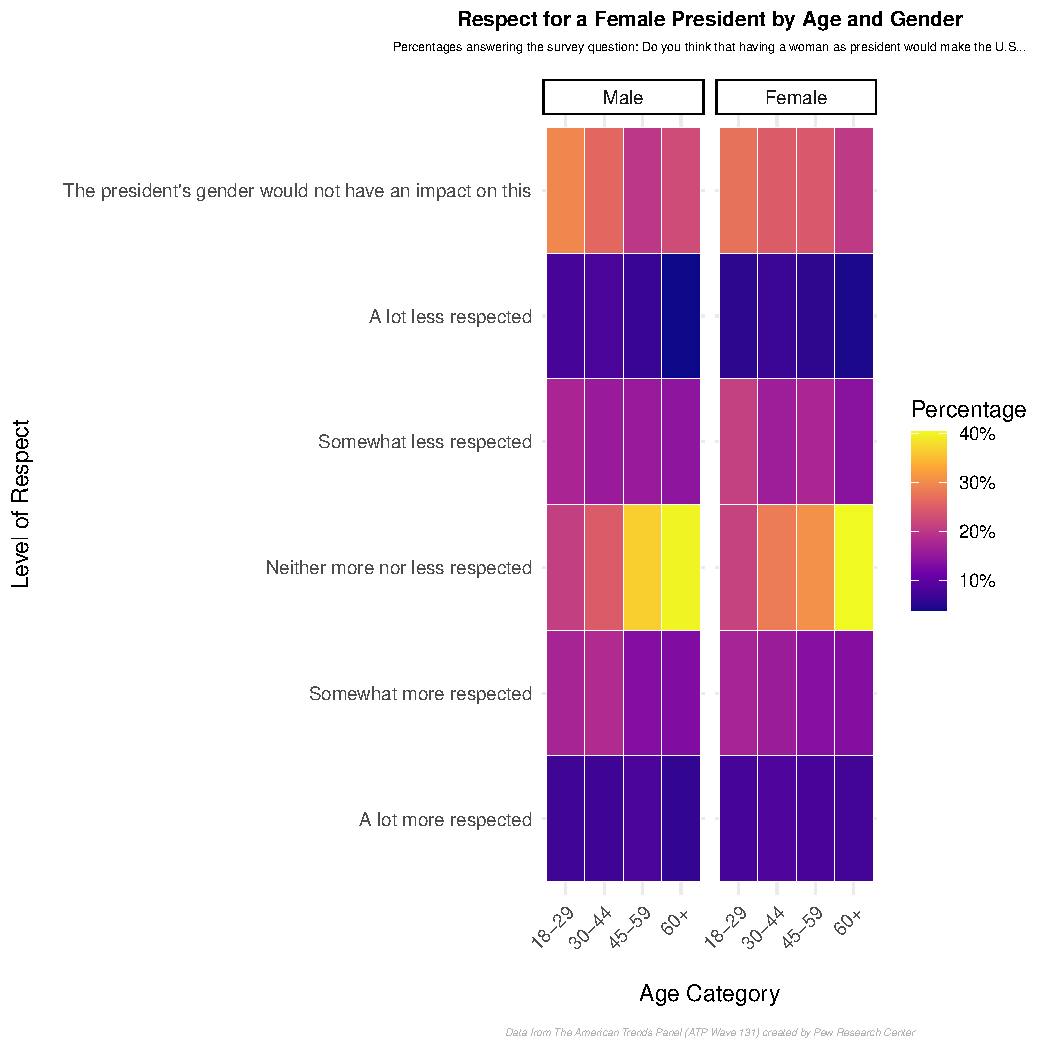
\includegraphics[width=0.9\textwidth]{heat.pdf}
\end{figure}

\title{Visualization 3}
\lstinputlisting[language=R, firstline=136, lastline=184]{final_project.R}  
\begin{figure}[H]
	\centering
	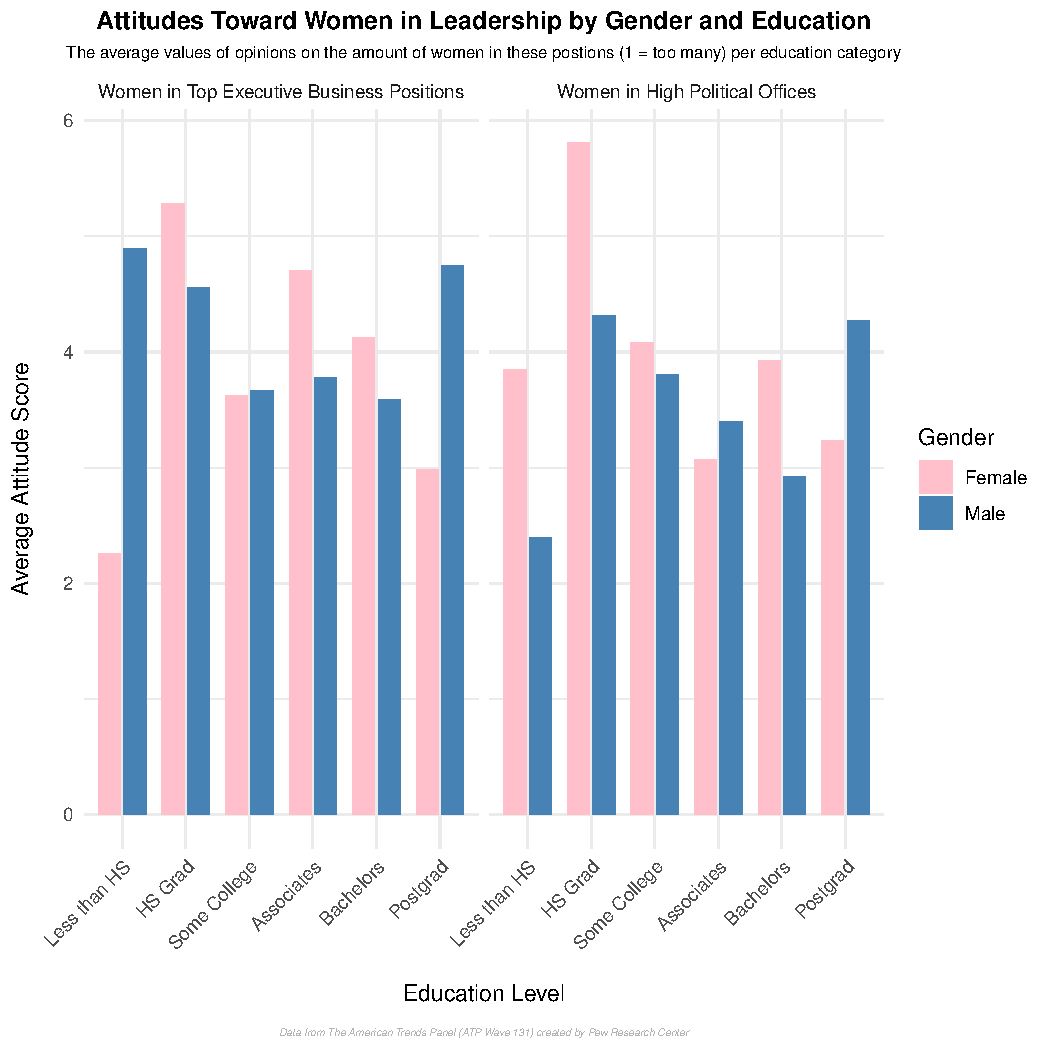
\includegraphics[width=0.9\textwidth]{bar_2.pdf}
\end{figure}
\end{document}
